
% =============================================================================



\chapter{Introduction}
In~the~software industry, the~accessible and~testable code is crucial for~modern
businesses, and~the~best way for~developers to~access or~test it is through
APIs\footnote{API is an~abbreviation for~an~Application Programming Interface
which is a~set of~protocols and~tools for~building application software.}. APIs
are supposed to~connect engineers, let companies add value to~their~products
and~create an~ecosystem of~shared knowledge that allows other developers to~use
the~functions provided by~the~interfaces. To~fulfill these tasks, the~interfaces
have to~be clear, accessible and~most importantly human and~machine readable. 
However, despite their importance, there hasn't been an~industry standard
for~documentating nor~testing them.

The~thesis aims to~solve the~problem of~testing the~applications interfaces.
The~goal is to~develop an~application having an~innovative user interface
with~regard to~clarity and~simple use, aimed to~developers, even in~case
of~large interfaces. The~application will be based on~Swagger framework, which
provides a~way to~automate API reference generation. The~resulting application,
called Restty, will provide not~only way to~test single API endpoints, but
mainly the~functionality to~create extensive test cases from~the~listed web
services.

The~thesis is organized as~follows. Chapter~\ref{Preliminaries} gives
definitions needed to~follow the~thesis and~explains web services and~RESTful
APIs in~detail. Chapter~\ref{Technologies} focuses on~technologies that were
used for~development of~the~Restty application. Chapter~\ref{Design} describes
the~application's designs and~mockups, which were used to~reveal any clashing
visual elements before writing the~code. The~second to~last
Chapter covers the~development of~Restty using the~technologies listed
in~previous sections and~testing the~application using the~API from~the~Red Hat
JBoss BPM Suite application. The~last Chapter contains an~overall summary
of~the~developed solution and~final thoughts on~the~work done within the~thesis.



% =============================================================================



\chapter{Preliminaries and Definitions}
\label{Preliminaries}
This chapter will gradually introduce terms necessary to~follow the~thesis.
In~the~first section is introduced basic terminology and~established notion
of~remote interfaces and~web services. In~the~next section is provided
an~explanation of~what APIs are and~the~last section covers the~importance
of~theirs testing.



\section{Understanding the Web Services}
\label{WebServices}
A~web service is a~software system designed to~support interoperable machine
to~machine interactions over~a~network. It is a~collection of~open protocols
and~standards used for~exchanging data between applications or~systems. Software
applications written in~various programming languages and~running on~various
platforms can use web services to~exchange data over~the~networks like
the~Internet in~a~manner similar to~interprocess communication on~a~single
computer.

In~the~past, web services used mostly SOAP\footnote{Simple Object Access
Protocol is a~protocol specification for~exchanging structured information
in~the~implementation of~web services in~the~computer networks.} over~HTTP
protocol~\cite{HTTP}, allowing less costly interactions over~the~Internet.
However, in~2004 the~W3C extended the~definition of~web services
about~\uv{REST-complient} web services~\cite{W3CWebServices}, in~which
the~primary purpose of~the~web service is to~manipulate XML or~JSON
representations of~web resources using a~uniform set of~stateless operations.



\subsection{Introduction to RESTful Web Services}
The~REST, abbreviation of~Representationl State Transfer, is an~architectural
style for~networked hypermedia applications, primarily used to~build web
services. The~term was first defined in~the~year~2000 by~R.~Fielding in~his
doctoral dissertation~\cite{FieldingDissertation}. In~the~dissertation, Fielding
explained that the~REST principles were known as~the~\uv{HTTP object model}
beginning in~1994, and~were used in~designing the~HTTP~1.1 and~Uniform Resource
Identifiers~\cite{URI-RFC} standards.

The~REST architectural style constrains an~architecture to~a~\uv{client-server}
architecture and~is designed to~use a~stateless communication protocol,
typically HTTP. A~client and~a~server exchange representations of~resources
by~using standardized interface and~a~protocol. When the~client accesses
the~resource using unique URI, a~representation of~the~resource is returned.
With~each new resource representation, the~client is said to~transfer state.
The~resources are typically represented by~text, JSON or~XML, while JSON being
currently the~most popular format being used.



\subsection{Messaging}
As~mentioned in~previous section, the~RESTful web services can use any stateless
communication protocol as~a~medium of~communication between client and~a~server.
However, the~HTTP protocol is the~most popular. The~communication works
as~follows: the~client sends a~message in~form of~HTTP~Request and~the~server
responds in~the~form of~HTTP Response. This technique is termed
as~\textit{Messaging}. Apart from~the~data, the~messages also contain some
metadata about the~message itself. As~can be seen
in~the~figure~\ref{fig-HTTPRequest} a~request message consists of~five major
parts.

\begin{figure}[!hbt]
	\centering
	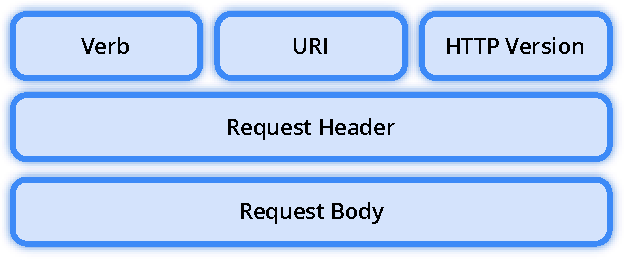
\includegraphics[width=0.5\textwidth]{./figures/http-request.pdf}
	\caption{The~format of~a~HTTP Request.}
	\label{fig-HTTPRequest}
\end{figure}

\begin{enumerate}
  \item Verb indicates the~HTTP method like GET, PUT, POST, etc.
  \item URI is the~Uniform Resource Identifier used to~identify the~resource
  on~the~server.
  \item HTTP version is the~version of~HTTP.
  \item Request header contains metadata as~a~collection of~\uv{key-value} pairs
  of~headers and~their values. For~instance, a~client (or~browser) type, format
  supported by~the~client, format of~the~message body, cache settings
  for~the~response, and~more.
  \item Request body is the~message content or~resource representation.
\end{enumerate}

In~the~listing~\ref{lst-GETRequest} can be seen an~example of~a~request that was
created by~the~browser when it tried to~access the~website of~Faculty
of~Information Technology.

\vspace{1mm}
\begin{lstlisting}[caption=An~example of~a~simplified GET request made
by~the~browser., label=lst-GETRequest, style=dp-default]
GET / HTTP/1.1
Host: www.fit.vutbr.cz
User-Agent: Mozzila/5.0 (Windows NT 6.3; Win64; x64) ...
Accept: text/html,application/xhtml+xml,application/xml; ...
Accept-Encoding: gzip, deflate
Accept-Language: cs-CZ,cs;
\end{lstlisting}

As~can be seen, the~HTTP method is followed by~the~URI and~the~HTTP version.
The~request also contains some headers. For~instance
the~\uv{\textit{User-Agent}} header contains information about the~type
of~a~client which made the~request. The~\textit{Accept} headers tells the~server
about various representation formats, the~encoding, and~a~language the~client
supports. The~server, if it supports more than one representation format, can
decide the~format for~the~response at~runtime depending on~the~value
of~the~\textit{Accept} header.

When the~server receives the~request it responds with~a~HTTP response which
consists of~four major parts as~can be seen
in~the~figure~\ref{fig-HTTPResponse}.

\begin{figure}[!hbt]
	\centering
	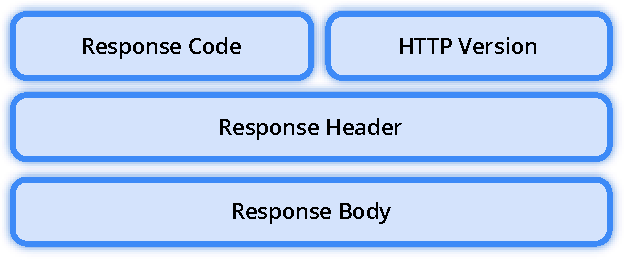
\includegraphics[width=0.5\textwidth]{./figures/http-response.pdf}
	\caption{The~format of~HTTP response.}
	\label{fig-HTTPResponse}
\end{figure}

\begin{enumerate}
  \item Response code contains the~server status for~the~requested resource.
  The~response is a~\uv{3-digit} status code, for~instance, 404 means resource
  not found and~200 means response is ok.
  \item HTTP version is the~version of~HTTP.
  \item Response header contains metadata and~settings of~the~response message
  as~\uv{key-value} pairs. For~example, content type, content language,
  response date, etc.
  \item Response body contains message content or~resource representation if
  the~request was successful.
\end{enumerate}

In~the~listing~\ref{lst-GETResponse} can be seen an~example of~a~response
to~a~request from~the~listing~\ref{lst-GETRequest}. The~response contains
the~version of~HTTP, response code and~several response headers followed
by~the~response body which in~this case is a~HTML page.

\vspace{1mm}
\begin{lstlisting}[caption=An~example of~a~simplified response to~GET
request., label=lst-GETResponse, style=dp-html]
HTTP/1.1 200 OK
Date: Sat, 09 Dec 2017 08:36:01 GMT
Server: Apache
Content-Location: index.php.cz
Pragma: no-cache
Keep-Alive: timeout=60, max=100
Connection: Keep-Alive
Transfer-Encoding: chunked
Content-Type: text/html; charset=iso-8859-2
Content-Language: cs
<!DOCTYPE HTML PUBLIC "-//W3C//DTD HTML 4.01//EN">
<html>
<head>
...
\end{lstlisting}



\subsection{Addressing the Resources}
\label{sec-addressing}
If the~client wants to~get a~resource from~the~server, it needs to~know, how
to~address it. \textit{Addressing} refers to~locating a~resource or~multiple
resources lying on~the~server. It is analogous to~locating a~postal address
of~a~person. A~RESTful service uses directory hierarchy like human readable URIs
to~address its resources. Each resource is identified by~its URI which is
of~the~following format:

\begin{equation}
<protocol>://<serviceName>/<resourceType>/<resourceId>
\end{equation}

However, it needs to~be noted that the~URI should not say anything about
the~operation or~action, because for~identifying the~operation to~be performed
on~the~resource, the~HTTP verbs are used. This enables the~client to~call
the~same URI with different verbs to~perform different operations. The~verbs
correspond to~read, create, update, and~delete\footnote{In~computer
programming, create, read, update, and~delete (as~an~acronym CRUD) are four
basic functions of~persistent storage.} operations. Nevertheless, while
designing URIs there are other practices that should be considered as~well.

\begin{enumerate}
  \item Plural nouns should be used to~define resources.
  \item Spaces should be avoided. Typically in~URIs it's recommended to~use
  underscore or~hyphen when using long resource name.
  \item Lowercase letters are recommended. Although URIs are
  \uv{case-insensitive}, it's a~good practice to~keep them in~lower case letters
  only.
  \item Avoid verbs for~the~resource name until the~resource is actually
  an~operation or~a~process.
\end{enumerate}



\subsection{HTTP Verbs}
\label{lab-verbs}
As~stated in~section~\ref{sec-addressing} the~most used HTTP verbs correspond
to~CRUD operations. For~instance, read operation corresponds to~the~GET verb
which is used to~retrieve a~representation of~a~resource. If the~request is
successful, it returns representation of~the~resource in~a~format that is
accepted by~the~client and~a~response code of~200. Note that the~requests that
utilize the~verb should be used only to~read data, not change it. When used this
way they are considered safe. That is, they can be called without risk of~data
modification or~corruption. Additionally, the~requests are idempotent, which
means that making multiple identical requests ends up having the~same result
as~a~single request.

For~creating resources, the~POST is most often utilized. On~successful creation,
returning a~\textit{Location} header, with a~link to~the~created resource,
and~the~201 response code. The~method is neither safe nor idempotent. Therefore
it is recommended for~\uv{non-idempotent} resource requests. Making two
identical POST requests will most likely result in~two resources containing same
information.

For~update capabilities, the~PUT verb is ofter most utilized, \uv{PUT-ing}
to~a~known resource with the~request body containing the~newly updated
representation of~the~original resource. On~successful update, the~server should
return the~200 or~204 status code if not returning any content in~the~body. It
follows from the~above that a~body in~the~response is optional -- providing one
is not necessary and~only leads to~more bandwidth consumption. The~PUT is not
a~safe operation, in~that it modifies state on~the~server, but is idempotent.
In~other words, if the~resource is updated using the~PUT method and~then
the~same call is made again, the~resource is still there and~has the~same state
as~it did with~the~first call.

The~DELETE verb is pretty straightforward, it is used to~delete a~resource.
On~successful deletion, the~server should return response code of~204 with no
response body. \uv{HTTP-spec-wise}, the~operations are idempotent. If
the~resource is deleted, it is gone. Repeatedly calling the~method on~that
resource ends up the~same -- the~resource is gone. However, there is a~caveat
about the~method's idempotence. Calling it on~the~resource a~second time will
result in~404 response code since the~resource was already removed and~therefore
is no longer findable. It makes the~operation in~fact no longer idempotent,
however, the~\uv{end-state} of~the~resource is the~same.



\subsection{Representation of the Resources}
It is clear that the~focus of~RESTful services is on~resources and~on~providing
access to~them. A~resource can easily be thought of~as~an~object
as~in~OOP\footnote{Object oriented programming (OOP) is a~programming paradigm
based on~the~concept of~\textit{objects}, which may contain data, in~the~form
of~fields; and~code, in~the~form of~procedures, often known as~methods.}.
The~resources can be text files, HTML pages, images or~videos and~can consist
of~other resources. The~server simply provides access to~the~resources
and~client accesses and~modifies them. It is important to~point out that
the~architecture does not put a~restriction on~the~format of~a~resource
representation. However, as~mentioned before, the~most popular representation
formats are XML and~JSON.

\vspace{1mm}
\begin{lstlisting}[caption=An~example of~a~XML representation
of~a~\textit{user} resource., label=lst-XMLExample, style=dp-xml]
<user>
	<id>1</id>
	<firstName>John</firstName>
	<lastName>Doe</lastName>
	<age>42</age>
</user>
\end{lstlisting}

Once a~resource is identified then its representation is to~be decided using
a~standard format so that the~server can send the~resource in~the~above said
format and~the~client can understand said format.

\vspace{1mm}
\begin{lstlisting}[caption=An~example of~a~JSON representation
of~a~\textit{user} resource., label=lst-JSONExample, style=dp-default]
{
	"id": 1,
	"firstName": "John",
	"lastName": "Doe",
	"age": 42
}
\end{lstlisting}

Despite the~fact that there are no restrictions on~the~format of~a~resource
representation, following some important points should be considered.
For~instance, both the~server and~the~client should be able to~understand said
format. Moreover the~format should be able to~represent the~resource completely.



\section{Introduction to~Application Programming Interfaces}
In~computer programming an~application programming interface is the~defined
interface through which interactions happen between an~enterprise and~users
of~its assets. It can become the~primary entry point for~enterprise service,
for~its own website and~applications, as~well as~for~a~partner and~customer
integrations. It is defined through a~contract so~that any application can use
it with relative ease. 

The~API~\cite{RESTfulAPI} approach creates a~loosely coupled architecture that
allows a~component service to~have a~wide range of~future uses, and~is
technology agnostic. The~architecture resolves around providing programmable
interfaces to~a~set of~services to~different applications serving different
kinds of~customers. It assumes that these user groups might change or~evolve
over time in~the~way they utilize the~provided services. The~strategy
of~providing APIs leads to~the~following benefits:

\begin{enumerate}
  \item With~APIs, computers rather than people can manage the~work. Through
  them, companies can update work flows to~make them quicker and~more
  productive.
  \item They allow content to~be embedded from~any site or~application more
  easily. This guerantees more fluid information delivery and~an~integrated user
  experience.
  \item Using APIs, any user or~company can customize the~content and~services
  that they use the~most.
  \item They represent a~cheaper way of~building applications by~increasing
  the~reuse of~services. Providing a~usage or~\uv{analytics-based} evolutionary
  development platform decreases cost of~development and~change to~services.
  \item The~company that releases the~API allows its customers to~access their
  conferencing services in~new, more efficient ways, increasing brand
  recognition and~customer loyalty.
\end{enumerate}



\subsection{When is API RESTful?}
The~previous sections explained the~principles of~RESTful web services
and~introduced the~term Application Programming Interface. However, it is
necessary to~point out that not all web APIs are considered RESTful. An~API is
RESTful only when it is acting under the~REST constraints at~all times. These
constraints restrict the~ways that the~server may process and~respond to~client
requests so~that, by~operating within these constraints, the~service gains
desirable \uv{non-functional} properties, such~as~performance, scalability,
portability and~reliability. These formal constraints are as~follows:

\begin{enumerate}
  \item \textbf{\uv{Client-Server}} -- the~constraint is based
  on~the~separation of~concerns principle. Separating the~user interface
  concerns from the~data storage concerns improves the~portability of~the~user
  interface across multiple platforms.
  \item \textbf{Stateless} -- communication between client and~server have~to be
  stateless. It means that each request from~client to~server must contain all
  the~necessary information to~complete the~transaction. The~main advantage
  of~this approach is that the~system is able to~scale better because the~server
  does not have to~store client state between requests.
  \item \textbf{Cacheable} -- the~constraint ensures that the~clients can cache
  response to~improve performance. \uv{Well-managed} caching partially
  or~completely eliminates some \uv{client-server} interactions, further
  improving scalability and~performance.
  \item \textbf{Uniform Interface} -- in~order to~have efficient caching
  in~a~network, components have~to be able to~communicate via a~uniform
  interface.
  The~definition of~uniform interface consists of~four other constraints,
  however most of~them can be found implemented in~the~HTTP protocol.
  \item \textbf{Layered System} -- in~a~layered system, intermediaries, such
  as~proxies can be placed between client and~server utilising the~web's uniform
  interface. The~main advantage is that intermediaries can then intercept
  \uv{client-server} traffic for~a~specific purposes; for~example caching.
  \item \textbf{Code On Demand} -- it is an~optional constraint and~it allows
  clients to~download programs for~\uv{client-side} execution. The~best examples
  for this are compiled components such~as~Java applets or~\uv{client-side}
  scripts such~as~JavaScript.
\end{enumerate}



\section{The~Importance of~API Testing}
\label{frameworks}
Software testing is an~important phase of~the~software development life cycle
in~general, with~API testing being one of~its most challenging
parts~\cite{TestingAPI}. It is being more~and~more recognised as~being more
suitable for~test automation and~continuous testing than other forms of~testing.
Many~developer teams are starting to~increase the~level of~API testing while
decreasing their reliance on~GUI testing because the~tests at~the~API layer are
less brittle and~easier to~maintain even thought they have to~cover
individual functionalities as~well~as~series or~chain of~functionalities.

In~general the~API testing is used to~determine whether the~APIs
and~the~integrations they enable work in~the~most optimal manner e.g. whether
they return the~correct response, react properly to~edge cases, delivery
responses in~an~acceptable amount of~time, and~respond securely to~potential
security attacks. On~particular, the~testing concentrates on~using software
to~make API calls in~order to~receive an~output before observing and~logging
the~system's response. This enables to~test if the~API returns a~correct
response or~output under varying conditions. The~output is typically a~pass
or~fail status, date, information or~a~call to~another API. However it is
important to~point out that there could be no output at~all or~something
completely unpredicted can occur.

Overall, it's very clear that the~risk of~putting a~bad and~especially insecure
product on~the~market is greater than the~cost to~test it which is why the~API
testing is crucial part of~the~application development process.



\subsection{Beginning with cURL}
As~APIs are becoming an~integral part of~how software works it is not
a~surprise that many frameworks and~applications for~theirs testing were
developed. Probably the~oldest of~them is cURL~\cite{cURL}. It is a~command line
tool for~transferring data using various protocols. It consists of~two products
--~libcurl and~curl. Libcurl is a~\uv{client-side} transfer library with~support
for~a~wide range of~protocols. It is portable, \uv{thread-safe}, feature rich,
and~well supported on~virtually any platform. On~the~other hand, curl is
a~command line tool for~getting or~sending files using URL syntax. Since curl
uses libcurl, it supports the~same range of~common Internet protocols that
libcurl does. In~general, it provides a~generic, language agnostic way
to~demonstrate HTTP requests and~responses.

In~addition, as~REST follows the~same model as~the web, it is possible to~type
an~HTTP address to~the~curl and~use it to~make an~HTTP request to~a~resource
on~a~server. The~server returns a~response, which would typically be converted
by~the~browser to~a~more visual display, as~a~raw code to~show the~developers
what they are really retrieving. Obviously, the~requests that can be made
with~the~tool may test various functionalities such as~sending requests using
various HTTP verbs, specifying query strings and~parameters or~even using
authentication.

\vspace{1mm}
\begin{lstlisting}[caption=An~example of~POST request that creates
\textit{user} resource on~the~server using API endpoint \textit{/users}.,
label=lst-cURL-POST, style=dp-no-strings, language=XML]
curl --request POST \
  --url https://localhost:8080/users \
  --header 'authorization: Bearer {{AcessToken}}' \
  -d '{
  	"firstName": "John", \ 
  	"lastName": "Doe", \
  	"age": 42 \
  }'
\end{lstlisting}

However, it is a~little cumbersome to~work directly with curl, since even
a~simple curl request may look like in~the~listing~\ref{lst-cURL-POST}.
Therefore, other frameworks and~applications, such as~Postman, were developed.



\subsection{Continuous Testing with Postman}
Postman is a~useful tool for~testing the~functionality of~API endpoints. It has
a~nice UI, which makes it easy to~add or~remove parameters, define headers,
authorization methods, and~data without the~hassle of~writing code. It also
allows developers to~create various environments, variables, and~to~save
requests, which curl is not designed to~do.

Besides providing a~friendly user interface for~constructing HTTP requests,
Postman also gives developers the~ability to~write tests against the~responses
of~requests to~see if the~server is returning the~correct results. Requests
constructed in~Postman can also be bundled into a~collection and~easily exported
or~shared, making Postman great for~collaborating on~and~sharing API
specifications with~other developers. In~addition, the~collections can also be
used with~continuous integration systems so that the~same collection used
to~test an~API locally while developing can also be used to~determine whether
or~not the~codebase should be pushed live onto production.

However, there is a~problem with~using Postman for~continuous testing,
because as~was stated in~the~section~\ref{lab-verbs}, not all HTTP verbs are
idempotent. To~clarify, what if a~developer creates a~test that removes
a~resource with~specified identifier from~a~database? If the~code covered
by~the~test is bugfree then the~resource is removed and~the~test successful.
Nevertheless, running the~test repeatedly will result in~the~test's failure
as~the~resource no longer exist. The~solution would be to~create a~test case
that calls the~endpoint which creates the~resource, and~then using the~resource
identifier from~the~response to~remove it. Unfortunately, Postman or~any other
similar application does not allow to~use request's response as~an~input
of~another request.



% =============================================================================



\chapter{Technologies and Frameworks}
\label{Technologies}
In~this chapter are discussed the~details of~technologies and~frameworks that
were used for~the~development of~the~Restty aplication. In~the first sections is
introduced the~Java language and~the~Spring and~Hibernate frameworks that were
used for~building the~backend of~the~application. Following the~thesis
the~frontend web application framework Angular along with~the~superset
of~EcmaScript~6 --~the~TypeScript language is presented, as~well~as~the~web
framework PatternFly and~its key features. Finally, the~last section covers
the~Swagger framework and~its usage within the~Restty application.



\section{Introduction to Java}
The~Java language project was initiated in~June 1991 by~J.~Gosling~\cite{Java}
for~use in~one of~his \uv{set-top} box projects. The~language, initially called
\textit{Oak}, ended up later being renamed as~Java when it was first publicly
released by~Sun Microsystems in~1995. The~language promised \uv{Write Once, Run
Anywhere} (WORA), meaning that compiled Java code can run on~all platforms that
support Java without the~need for~recompilations.

The~WORA is achieved by~compiling the~Java language code to~an~intermediate
representation called Java bytecode, instead of~compiling the~code directly
to~architecture specific machine code. When compiled, the~bytecode is executed
by~a~Java Virtual Machine, which is a~separate program that is optimized
for~the~specific platform on~which the~Java code is run.

\begin{figure}[!hbt]
	\centering
	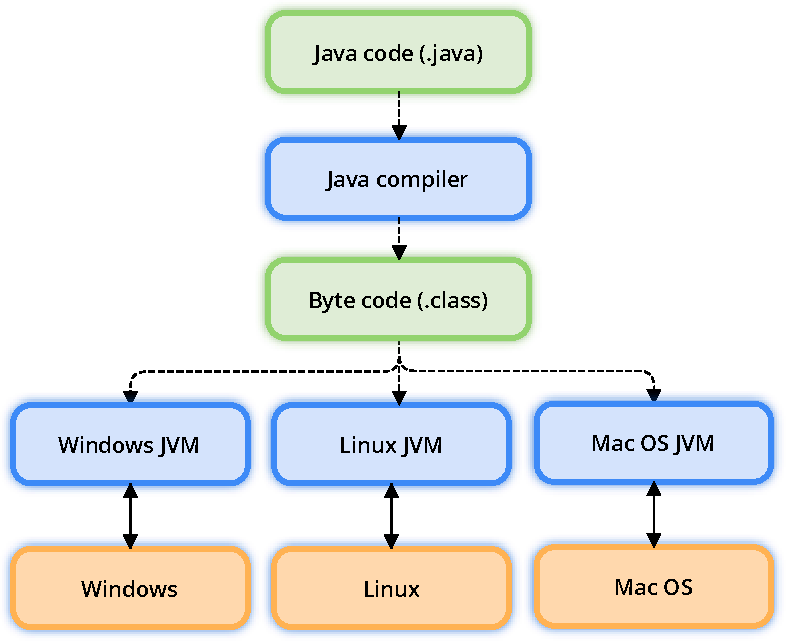
\includegraphics[scale=0.7]{./figures/java-jvm.pdf}
	\caption{Illustration how Java ensures the~\uv{Write Once, Run Anywhere}
	property.}
\end{figure}

However, the~Java's portability is not its only advantage over~other languages
that can be used to~build backend of~a~web application. For~instance, among
the~other benefits belongs the~automatic storage management, strong typing, 
flexible namespace, or~standards for~connectivity to~relational databases.

To~clarify, automatic storage management means that the~JVM automatically
performs all memory allocation and~deallocation while the~program is running.
The~developers cannot explicitly allocate memory for~new objects or~free memory
for~objects that are no longer referenced. Instead, they depend on~a~JVM
to~perform these operations. The~process of~freeing memory is known as~garbage
collection.

In~addition, Java's flexible namespace makes it perfect for~writing complex
applications. That is because Java defines classes and~places them within
a~hierarchical structure that mirrors the~domain namespace of~the~Internet,
which avoids name collisions and~allows Java applications to~be distributed. 



\subsection{Basics of~Java's syntax}
The~syntax of~Java is largely influenced by~C++. However, unlike C++, which
combines the~syntax for~structured, generic, and~\uv{object-oriented}
programming, Java was built almost exclusively as~an~\uv{object-oriented}
language. All code is written inside classes, and~every data item is an~object,
with~the~exception of~the~primitive data types such~as~integers, characters
and~boolean values, which are not objects for~performance reasons.

Following the~above, a~Java program can be defined as~a~collection of~objects
that communicate via invoking each other's methods. To~clarify, object is
an~instance of~a~class, which is a~template that describes the~behavior
and~state that the~object of~its type supports. The~behavior is described via
methods, where the~logics are written, data is manipulated and~all the~actions
are executed.

Nevertheless, as~was mentioned above, Java was influenced by~C++ therefore it is
not a~surprise that the~syntax is similar. However, there are some differences.

\begin{enumerate}
  \item Java is case sensitive, which means identifier \textit{Hello}
  and~\textit{hello} would have different meaning in~Java.
  \item For~all class names, the~first letter should be in~upper case. If
  several words are used to~form a~name of~the~class, each inner word's first
  letter should be in~upper case.
  \item All method names should start with a~lower case letter. If several words
  are used to~form the~name of~the~method, then each inner word's first letter
  should be in~upper case.
  \item Name of~the~class file should exactly match the~class names. That is
  because if~the~file name and~the~class name do not match, the~program will not
  compile.
\end{enumerate}

Overall the~Java's syntax and~best practices are quite extensive, starting
with~basics like identifiers, modifiers, arrays or~interfaces and~ending
with~more advanced features like generics, annotations and~lambda expressions
that were added to~the~language specification over~the~years. Unfortunately,
these specifications are not the~subject of~the~thesis to~be explained
in~detail.



\section{Building a RESTful Web Service}
Even though Java is powerful language, building a~backend of~an~enterprise
application in~plain Java is no easy task. Fortunately, there are many libraries
and~frameworks that provides a~way of~creating high performing, testable web
applications with ease. One of~the~most popular is~the~Spring
Framework~\cite{Spring}, which is an~open source Java platform, initially
released in~June 2003. Spring can be used for~development of~any Java
application, but shines when used for~building web applications on~top
of~the~Java~EE platform. Spring targets to~make J2EE development easier to~use
and~promotes good programming practices by~enabling
a~\uv{POJO-based\footnote{In~software engineering, a~Plain Old Java Object
(POJO) is an~ordinary Java object, not bound by~any special restriction and~not
requiring any class path.}} programming model.



\subsection{The~Advantages of Using Spring Framework}
First and~foremost, the~technology that Spring is most identified with~is
the~Dependency Injection (DI) flavor of~Inversion of~Control (IoC). The~IoC is
a~general concept, and~it can be expressed in~many different ways. Dependency
Injection is merely one concrete example of~IoC.

When writing complicated Java application, the~application classes should be
as~independent as~possible of~other Java classes to~increase the~possibility
to~reuse these classes and~to~test them independently of~other classes while
unit testing. Dependency Injection helps in~gluing these classes together
and~at~the~same time keeping them independent. To~clarify, consider
an~application which has a~text editor component and~the~developer wants
to~provide a~spell check to~said component. The~standard code would look similar
to~the~code in~the~listing~\ref{lst-spring-di-1}, creating a~dependency between
\textit{TextEditor} and~the~\textit{SpellChecker} classes.

\vspace{1mm}
\begin{lstlisting}[caption=The~standard way of~providing spell checking
to~a~component., style=dp-default, language=Java, label=lst-spring-di-1] 
public class TextEditor {

	private SpellChecker spellChecker;
	
	public TextEditor() {
		this.spellChecker = new SpellChecker();
	}
	
}
\end{lstlisting}

As~can be seen in~the~listing~\ref{lst-spring-di-2}, in~an~inversion of~control
scenario, the~developer would create code differently, in~this scenario
the~total control was removed from~the~\textit{TextEditor} class
and~the~dependency (i.e. \textit{SpellChecker} class) is being injected into
the~\textit{TextEditor} through a~class constructor. Thus the~flow of~control
has been \uv{inverted} by~Dependency Injection because the~developer effectively
delegated dependencies to~an~external system.

\pagebreak
\begin{lstlisting}[caption=The~Inversion of~Control scenario of~providing
a~\textit{SpellChecker} to~the~\textit{TextEditor} component., style=dp-default,
language=Java, label=lst-spring-di-2]
public class TextEditor {

	private SpellChecker spellChecker;
	
	public TextEditor(SpellChecker spellChecker) {
		this.spellChecker = spellChecker;
	}
	
}
\end{lstlisting}

The~other key~advantage of~Spring is the~Aspect Oriented Programming (AOP)
framework. AOP entails breaking down program logic into distinct parts called
concerns. The~functions that span multiple points of~an~application are called
\uv{cross-cutting} concerns and~are conceptually separate from~the~application's
business logic. As~mentioned earlier, the~key unit of~modularity in~OOP is
the~class, whereas in~AOP the~unit of~modularity is the~aspect, which is
the~combination of~the~pointcut and~the~advice~\footnote{Advice describes
a~class of~functions which modify other functions when the~latter are run.}.
As~DI helps decouple the~application objects from~each other, AOP helps decouple
\uv{cross-cutting} concerns from~the~objects that they affect. To~clarify,
the~AOP module provides interceptors to~intercept an~application meaning when
a~method is executed, the~developers have the~option to~add an~extra
functionality before or~after the~method execution using the~interceptors.



\section{Persisting Data With Hibernate}
Even though the~Spring Framework covers a~lot of~functionality needed to~build
complex web application and~adds significant enhancements to~the~data access
layer of~Java language, it is still best to~use external
ORM\footnote{\uv{Object-relational} mapping (ORM) is a~programming technique
for~converting data between incompatible type systems using
\uv{object-oriented} programming languages.} framework. For~the~development
of~the~Restty application I've chosen to~use the~Hibernate
framework~\cite{Hibernate} on~top of~the~H2 database.

Hibernate is a~high performance ORM solution for~Java, created by~G.~King
in~2001. Hibernate maps Java classes to~database tables ~Java data types to~SQL
data types and~relieves the~developer from~most of~common data persistence
related programming tasks. Hibernate consists of~layered architecture which
helps the~developer to~operate without having to~know the~underlying APIs. It
makes use of~the~database and~configuration data to~provide persistence services
(and~persistent objects) to~the~application. The~entire concept of~Hibernate is
to~take the~values from~Java class attributes and~persist them to~a~database
table. To~provide such functionality, the~classes should follow specific rules.

\begin{enumerate}
  \item A~class that will be persisted needs a~default constructor.
  \item All classes should contain an~ID in~order to~allow easy identification
  of~the~objects within Hibernate and~the~database. The~ID property is mapped
  to~the~primary key of~a~database table.
  \item All attributes that will be persisted should be declared private
  and~have appropriate getters and~setters defined in~the~JavaBean style.
\end{enumerate}

\begin{figure}[!hbt]
	\centering
	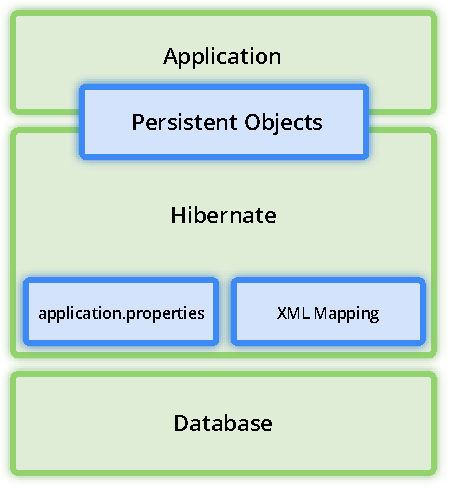
\includegraphics[scale=0.8]{./figures/hibernate-architecture.pdf}
	\caption{High level view of~the~Hibernate framework architecture.}
\end{figure}

As~can be seen in~the~listing~\ref{lst-table}, a~class is mapped to~the~database
using Hibernate annotations on~the~entity. Hibernate's annotations are a~way
of~providing the~metadata for~the~ORM mapping. All the~metadata is clubbed
into~the~POJO Java file along with~the~code, which helps the~developer
to~understand the~table structure and~POJO simultaneously during
the~development.

\vspace{1mm}
\begin{lstlisting}[caption=POJO class that features the~advantages of~ORM.,
style=dp-default, language=Java, label=lst-table]
@Entity
@Table("users")
@SequenceGenerator(name = "users_id_sequence", allocationSize = 1)
public class User {

	private Long id;
	private String name;
	
	@Id
	@Column(name = "id")
	@GeneratedValue(strategy = SEQUENCE, generator = "users_id_sequence")
	public Long getId() {
		return id;
	}
	
	public void setId(Long id) {
		this.id = id;
	}
	
	@Column(name = "name")
	public String getName() {
		return name;
	}
	
	public void setName(String name) {
		this.name = name;
	}

}
\end{lstlisting}

When mapping the~entity, Hibernate detects the~annotations and~accesses
the~properties through getter and~setter methods by~default. The~primary key
of~the~table is determined by~the~\textit{@Id} annotation, which by~default will
automatically determine the~most appropriate primary key generation strategy
to~be used. However, the~default generation strategy can be overriden
by~applying the~\textit{@GeneratedValue} annotation, which takes two
parameters~--~strategy and~generator.

\vspace{1mm}
\begin{lstlisting}[caption=The~SQL code that is generated by~Hibernate when
mapping the~entity from~the~listing~\ref{lst-table}, style=dp-default,
language=SQL, label=lst-table-sql]
CREATE TABLE public.users
(
	id bigint NOT NULL,
	name character varying(255,
	CONTRAINT users_pky PRIMARY KEY (id)
)
\end{lstlisting}

The~second advantage of~using Hibernate is Hibernate Query Language (HQL) which
is an~\uv{object-oriented} query language, similar to~SQL, but instead
of~operating on~tables and~columns, HQL works with~persistent objects and~their
properties. The~queries are translated by~Hibernate into~conventional SQL
queries, which in~turns perform an~action on~the~database. Although it is
possible to~use SQL statements directly with~Hibernate's Native SQL, it is not
recomennded because of~possible database portability hassles and~Hibernate's SQL
generation and~caching strategies.

\vspace{1mm}
\begin{lstlisting}[caption=An~example of~HQL query that selects users with~name
\uv{John Doe}., style=dp-default, language=Java, label=lst-hql] 
StringBuilder hql = new StringBuilder(" FROM ");
hql.append(User.class.getName());
hql.append(" WHERE name = :name ");

Query query = session.createQuery(hql.toString());
query.setString("name", name);
return query.list();
\end{lstlisting}



\section{What is Angular?}
Angular~\cite{Angular} is an~open source TypeScript framework used to~build web
applications in~HTML and~TypeScript. It makes it easy to~build an~application
as~it combines declarative templates, dependency injection, \uv{end-to-end}
tooling, and~integrated best practices to~solve development challenges.


\subsection{Beginning as AngularJS}
Angular originally started as~AngularJS, it was developed in~2009
by~M.~Hevery~\cite{HeveryAngularJS} as~the~software behind an~online JSON
storage service that would have been priced by~the~megabyte,
for~\uv{easy-to-make} applications for~the~enterprise. However, the~business
idea was soon abandoned and~AngularJS was released as~an~open source library
in~October 2010.

The~framework was used to~overcome obstacles encountered while working
with~Single Page applications\footnote{A~single page application (SPA) is a~web
application or~web site that interacts with the~user by~dynamically rewriting
the~current page rather than loading entire new pages from a~server.}.
However, because some of~the~core assumptions in~AngularJS needed to~be changed,
in~September 2016 saw the~light of~the~day a~complete rewrite of~AngularJS.
Originally, the~rewrite was called \uv{Angular 2} by~the~team that built it, but
this led to~confusion among developers. To~clarify, the~team announced that
separate terms should be used for~each framework with \uv{AngularJS} referring
to~the~1.X versions and~\uv{Angular} without the~\uv{JS} referring to~version~2
and~up.

As~the~new version of~the~framework was developed, some new concepts appeared.
In~addition to~better \uv{event-handling} capabilities, powerful templates,
and~better support for~mobile devices, Angular introduced several new features.

\begin{enumerate}
  \item The~earlier version of~Angular had a~focus of~controllers, but now has
  changed the~focus to~having components over controllers. Components help
  to~build applications into many modules which helps in~better maintaining
  the~application over~a~period of~time.
  \item The~newer version of~Angular is based on~TypeScript which is a~superset
  of~JavaScript, maintained by~Microsoft. More information about TypeScript will
  be provided later in~the~section~\ref{TypeScript}.
  \item The~newer version of~Angular introduced services which are a~set of~code
  that can be shared by~different components of~an~application. For~instance,
  consider a~data component that picks data from~a~database, it is possible
  to~have it as~a~shared service that could be used across multiple
  components.
\end{enumerate}


\subsection{Angular's Core Concepts}
As~mentioned in~previous section, Angular introduces the~two core concepts
--~components and~services, respectively the~dependency injection. An~Angular
application will always have a~root component that contains all other
components. In~other words, an~application will always have a~component tree,
in~which components are~a~logical piece of~code that consists of~following
parts:

\begin{enumerate}
  \item Templates that are used to~render the~view for~the~application. They
  contains the~HTML that needs to~be~rendered as~well as~the~bindings
  and~directives.
  \item Classes that are like a~classes defined in~any language, such~as~C,
  except they are defined in~TypeScript. Classes contains properties, methods,
  and~the~code which is used to~support the~view.
  \item Metadata that contains an~extra data defined for~the~Angular class. They
  are defined using a~decorator.
\end{enumerate}

To~clarify, consider an~example from~the~listing~\ref{lst-angular-component}
which contains all three parts. It defines a~class called
\textit{HelloWorldComponent} which contains only one property --~\textit{title}.
The~component is then defined using the~\textit{@Component} decorator that
contains HTML template which is the~view that needs to~be rendered
in~the~application.

\pagebreak
\begin{lstlisting}[caption=An~Angular class with~the~\textit{@Component}
decorator and~a~HTML template., label=lst-angular-component, style=dp-default,
language=Java]
@Component ({
	selector: 'my-app-hello-world',
	template: `
		<div>
			<h1>{{title}}</h>
		</div>
	`,
})
export class HelloWorldComponent {
	title: string = 'Hello World!';
}
\end{lstlisting}

The~second cornerstone of~an~Angular application is dependency injection.
The~idea behind it is pretty simple. If a~component that depends on~a~service is
needed, the~developers do not create the~service by~themselves. Instead they
request one in~the~constructor and~the~framework will provide one. This approach
leads to~more decoupled code which enables testability and~easier maintainence.

\begin{figure}[!hbt]
	\centering
	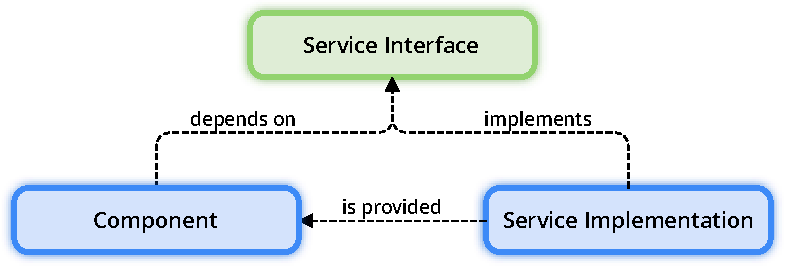
\includegraphics[scale=0.8]{./figures/dependency-injection.pdf}
	\caption{Angular's way of~injecting and~instantiating services
	in~the~components.}
	\label{fig-dependency-injection}
\end{figure}

To~clarify, consider an~example from~the~listing~\ref{lst-angular-service}.
The~listing contains a~simplified service that has a~method that returns
an~array of~users. If a~component is created and~an~argument
of~type~\textit{UserService} is passed to~the~component's constructor
as~a~parameter, Angular automatically instantiates and~injects the~service
into~the~component. 

As~can be seen, the~Angular's dependency injection module is flexible, and~easy
to~use because the~objects can be injected only via constructors. In~addition,
the~injectors form a~hierarchy, and~the~injectable object does not have to~be
an~\uv{application-level} singleton as~it might by~default in~Spring
framework\footnote{Spring framework is an~application framework and~inversion
of~control container for~the~Java platform that relies heavily on~dependency
injection.}.
\pagebreak

\begin{lstlisting}[caption=An~example of~dependency injection in~Angular.,
label=lst-angular-service, style=dp-default, language=Java]
export class UserService {
	users: User[] = [];
	
	findUsers(): User[] {
		// Code used to retrieve the users
		return users;
	}
}


@Component {
	...
}
export class UsersComponent {
	users: User[] = [];
	
	constructor(userService: UserService) {
		this.users = userService.findUsers();
	}
}
\end{lstlisting}


\section{Introducing~TypeScript}
\label{TypeScript}
In~september 1995 was first introduced JavaScript as~a~language for~the~client
side. It was used to~make webpages interactive and~to~provide online programs,
including video games. However, as~JavaScript code grows, it tends to~get
messier, making it difficult to~maintain and~reuse. Moreover, its failure
to~embrace the~features of~Object Orientation, strong type checking
and~\uv{compile-error} checks prevent JavaScript from~succeeding
at~the~enterprise level as~a~\uv{full-fledged} server side technology.
TypeScript was presented to~bridge this gap. Its main goals were to~provide
an~optional type system and~planned features from~future JavaScript editions
to~current JavaScript engines.


\subsection{Why Add Types to JavaScript}
Types have proven ability to~enhance code quality and~understandability.
Increasing the~agility when doing refactoring and~being one of~the~best forms
of~documentation a~developer can have. However, types have a~way of~being
unnecessarily ceremonious. Therefore TypeScript is very particular about keeping
the~barrier to~entry as~low as~possible, only providing compile type safter
for~the~JavaScript code. The~great thing is that the~types are completely
optional.

TypeScript provides data types as~a~part of~its optional type system. As~a~super
type of~all types, the~\textit{any} data type is used. It denotes a~dynamic type
and~using it is equivalent to~opting out of~type checking for~a~variable. That
suggests that the~variable may be declared with no type which means that
the~type of~the~varible will be inferred by~the~TypeScript Language Service.
All~other \uv{built-in} types and~\uv{user-defined} types inherit
from~the~\textit{any} type.

Important to~mention is that the~\uv{built-in} types \textit{undefined}
and~\textit{null} may look similar but are not the~same. A~variable initialized
with~\textit{undefined} means that the~variable has no value or~object assigned
to~it, while \textit{null} means that the~variable has been set to~an~object
whose value is undefined.

\begin{figure}[!hbt]
	\centering
	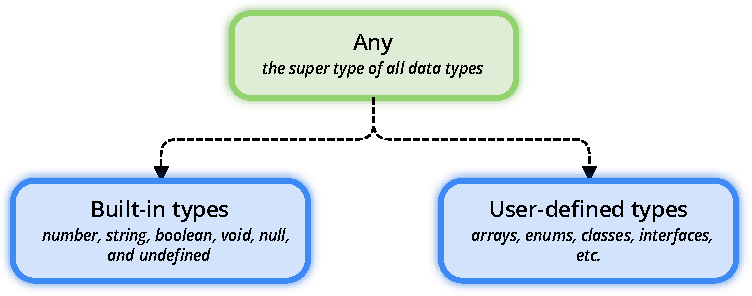
\includegraphics[scale=0.8]{./figures/data-types.pdf}
	\caption{Classification of~data types in~TypeScript.}
	\label{fig-datatypes}
\end{figure}

The~main advantage is however that the~JavaScript code files with the~\uv{.js}
suffix can be renamed to~a~files with \uv{.ts} suffix and~TypeScript will give
back a~valid equivalent to~the~original JavaScript file. That is because
TypeScript is intentionally and~strictly a~superset of~JavaScript with~optional
type checking.


\subsection{Future JavaScript}
The~second goal of~TypeScript was to~provide planned features from~future
JavaScript editions. Nowadays, it provides a~number of~features that are planned
in~EcmaScript~6\footnote{The~EcmaScript specification is a~standardized
specification of~a~scripting language.} for~current JavaScript engines.
For~instance, the~language features modules and~\uv{class-based} orientation
as~well as~features like generics and~type annotations that are not part
of~the~specification.

In~conclusion, even thought we could use JavaScript with Angular, TypeScript
feels like a~superior choice, not only because it is strongly typed and~supports
object oriented programming, but because of~the~TypeScript's transpiler which
provides the~\uv{error-checking} feature. Unlike JavaScript,
the~TypeScript is not an~interpreted language and~will compile the~code
and~generate compile errors if it finds some sort of~syntax errors. Thus
helps to~highlight the~errors before the~script is run hence, saving time trying
to~find the~bugs in~the~code.


\section{Styling with PatternFly}
The~success of~an~application depends on~a~\uv{well-designed} user interface.
The~good or~bad design can influence the~perceived usability of~an~application,
and~if the~application's design is not done well, whole application can be
perceived as~bad. The~PatternFly framework was developed specifically to~address
the~issue.

One of~the~main things that sets the~framework apart from~other libraries, such
as~Bootstrap, is the~focus on~design for~IT enterprise applications. It
recognizes the~importance for~a~user to~be able to~migrate seamlessly from~one
product to~another without having to~relearn the~UI. Behavioral consistency
leads to~better usability because users are familiar with~the~interactions.
Visual consistency establishes a~look and~feel that users recognize and~allows
to~unify disparate projects, make them look great and~make them look like they
belong in~the~same portfolio.

PatternFly is an~open source project that is based
on~Bootstrap~\cite{Bootstrap}, a~\uv{mobile-first} frontend framework
for~creating web sites and~applications. It is developed using Less, a~cascading
style sheet \uv{pre-processor} that extends the~CSS language and~adds features
that allow variables, mixins, functions, and~other techniques that allow
developers create code that is maintainable, themeable and extendible. This
allows the~developers to~add any required \uv{app-specific} CSS directly into
one CSS file, which is more performant, and~make any necessary adjustments
to~PatternFly via variable overrides.

The~framework consists of~a~series of~Less stylesheets that implements various
components of~the~toolkit. The~stylesheets are generally compiled into a~bundle
and~included in~the~applications, however individual components can be included
or~removed. Moreover, the~framework provides a~number of~variables that control
styling of~various components. Each component consists of~a~HTML structure
and~CSS declarations, and~in~some cases accompanying JavaScript code.


\subsection{Using the Components}
The~framework comes by~default with various design templates for~typography,
tables, forms, buttons, and~other interface components that can be used building
the~application --~saving lots of~time and~efforts in~the~development process.
The~templates are made available as~\uv{well-factored} CSS classes that
the~developers can apply to~the~HTML to~achieve different effects. By~using
semantic class name like \textit{.alert} or~\textit{.alert-success},
the~components are easily reusable and~extensible. Although PatterFly uses
descriptive class names that have a~meaning, it is not specific
about~implementation details. Therefore all classes can be overriden with~custom
style and~still, the~meaning of~the~class will remain the~same.

\begin{lstlisting}[caption=An~example of~styling the~component using predefined
class \textit{.alert}., label=lst-alert, style=dp-html]
<div class="container">
	<div class="alert alert-success">
		<span class="pficon pficon-ok"></span>
		<strong>Hello World!</strong>
		<span>This is an example of an alert in PatternFly.</span>
	</div>
</div>
\end{lstlisting}

As~can be seen in~the~figure~\ref{fig-alert}, the~code snippet
from~the~listing~\ref{lst-alert} generates a~component that contains
the~\uv{Hello World!} text. Using the~semantic class names, the~code is easily
styled, allowing the~developer to~spend more time on~application specific
features and~functions rather than application designs.

\begin{figure}[!hbt]
	\centering
	
\includegraphics[scale=0.8]{./figures/patternfly-alert.pdf}
	\caption{Illustration of~a~component styled using the~semantic classes
	from~PatternFly.}
	\label{fig-alert}
\end{figure}

\subsection{Working with the Grid}
In~the~beginning of~this section was mentioned that the~PatternFly, respectively
its predecessor Bootstrap, was developed with~a~\uv{mobile-first} design
philosophy, which resulted in~a~framework that is responsive by~design. The~end
result is that it easily and~efficiently scales with~a~single code base,
from~phones, through tablets, to~desktops. The~responsiveness is achieved using
a~fluid grid system that can be applied to~appropriately scale~up to~12 columns
according to~the~size of~the~device or~viewport. The~grids provides structure
to~the~layout, defining the~horizontal and~vertical guidelines for~arranging
content and~enforcing margins.

To~use the~grid system, a~few rules have to~be followed. Grid column elements
have to~be placed inside row elements, which creates horizontal groups
of~columns. It is possible to~have as~many rows as~needed, but it is necessary
that the~columns are immediate children of~rows. In~a~full row, the~column
widths are any combination that adds up~to~12, however it is not mandatory
to~use all~available columns.

\begin{lstlisting}[caption=An~illustration of~the~grid system in~PatternFly.,
label=lst-grid, style=dp-html]
<div class="container">
	<div class="row">
		<div class="col-md-6">First column</div>
		<div class="col-md-6">Second column</div>
	</div>
	<div class="row">
		<div class="col-md-3">First column</div>
		<div class="col-md-3">Second column</div>
		<div class="col-md-3">Third column</div>
		<div class="col-md-3">Fourth column</div>
	</div>
</div>
\end{lstlisting}

The~rows have to~be places in~a~\uv{fixed-width} layout wrapper that has
a~\textit{.container} class attached and~a~width of~1170px or~in~\uv{full-width}
layout wrapper, which has~\textit{.container-fluid} class attached, and~which
enables the~responsive behavior in~that row. The~grid system is based on~four
tiers of~classes -- \textit{xs} for~phones, \textit{sm} for~tables, \textit{md}
for~desktops, and~\textit{lg} for~larger desktops. These classes define
the~sizes at~which the~columns collapse or~spread horizontally. 


\section{Introduction to Swagger Framework}
Swagger~\cite{Swagger} is an~open source framework for~designing and~describing
APIs. It was developed by~Reverb Technologies in~2010 to~solve the~need
for~keeping the~API design and~documentation in~sync. It provides a~large
ecosystem of~tools that helps developers design, build, document, consume,
and~test RESTful web services. It defines a~standard, language agnostic
interface to~APIs which allows both humans and~machines to~discover
and~understand the~capabilities of~the~service. The~standard is called
the~OpenAPI Specification which is a~specification for~\uv{machine-readable}
interface files. The~files are essentially a~resource listings of~the~API which
adheres to~the~specification. The~files are either of~YAML or~JSON format
and~contains a~detailed description of~the~entire API. Nowadays there are two
ways to~create such file.

\begin{enumerate}
  \item \uv{Top-down} approach, or~\uv{design-first} which means using Swagger
  to~design the~API before writing any actual code.
  \item \uv{Bottom-up} approach, or~\uv{code-first} which means using Swagger
  to~document the~API of~an~existing code.
\end{enumerate}


\subsection{Using the~Swagger}
In~the~past, it was popular to~use the~\uv{code-first} approach which is much
easier because the~developers can make adjustmens on~the~fly, and~it fits nicely
into an~Agile delivery process. But because very often, the~developers are not
thinking about the~design, it can make the~API difficult to~understand
and~document. To~solve this, Swagger supports various annotations, as~can be
seen in~the~listing~\ref{lst-swagger-api}, that allow developers to~specify
the~details of~the~documentation. The~alternative way is to~let Swagger figure
out the~documentation by~itself based on~the~annotations from~Spring
framework\footnote{Swagger is~a~specification, and~supports a~wide range
of~frameworks and~their annotations.}. Under the~hood, it scans Spring
controllers on~\uv{start-up} and~registers a~documentation controller that
exposes the~operations Spring controllers implement. The~documentation follows
the~specification --~any client that understands the~specification can use
the~API. The~important thing is that the~documentation is based on~the~code
itself, therefore any change to~the~code is reflected on~the~documentation.
There is no need to~maintain an~external document.

\vspace{1mm}
\begin{lstlisting}[caption=An~example of~Spring controller with Swagger's
annotations that can be used to~generate API documentation., style=dp-default,
language=Java, label=lst-swagger-api]
@RestController
@RequestMapping("/users")
@Api(value = "users", description = "Users endpoints")
public class UserController {

	@Autowired
	private UserService userService;
	
	@GetMapping
	@ResponseStatus(HttpStatus.OK)
	public List<User> findAll() {
		return userService.findAll();
	}
	
	@PostMapping
	@ResponseStatus(HttpStatus.CREATED)
	public User create(@RequestBody UserDto userDto) {
		return userService.create(userDto);
	}
	
	@DeleteMapping
	@ResponseStatus(HttpStatus.NO_CONTENT)
	@RequestMapping(value = "/users/{userId}")
	public void remove(@PathVariable Long userId) {
		userService.removeById(userId);
	}

}
\end{lstlisting}

On~the~other hand, the~push for~clear, easy to~read documentation has
popularized the~\uv{design-first} approach. Not only more developers can have
input on~the~documentation, but it actually results in~cleaner code, because
the~developers are forced to~think simpler, more concise, and~easy to~follow.
The~framework contains an~editor that allows to~write up~the~documentation
in~appropriate formats and~have it automatically compared against the~Swagger
specification. Any mistakes are flagged, and~alternatives are suggested. This
way, when developers publish the~documentation they can be sure that it's
\uv{error-free}. As~can be seen in~the~listing~\ref{lst-swagger-json},
the~documentation consists of~2 parts, the~operations and~the~models.

In~either case the~framework exposes the~endpoints from~the~documentation
controller and~makes them accessible which allow for~applications to be built
upon the~documentation. The~application that will be developed in~the~thesis
will take an~advantage of~the~exposure. It will take an~existing JSON document
created by~the~framework and~build an~interactive documentation and~testing
environment upon it.

\vspace{1mm}
\begin{lstlisting}[caption=An~example of~API documentation in~JSON format
created using the~Swagger framework., style=dp-default, label=lst-swagger-json]
{
	"apiVersion": "1.0",
	"swaggerVersion": "1.0",
	"basePath": "http://localhost:8080",
	"resourcePath": "/users",
	"apis": [
		{
			"path": "/users",
			"description": "Users endpoints",
			"operations": [
				{
					"httpMethod": "GET",
					"summary": "findAll",
					"deprecated": "false",
					"responseClass": "List[User]", 
				},
				
				... 
			]
		}
	],
	"models": [
		"User": {
			"properties": {
				"id": {
					"type": "long"
				},
				"firstname": {
					"type": "string"
				},
				"lastname": {
					"type": "string"
				}
			}
		}
		
		...	
	]
}
\end{lstlisting}
  


% ==============================================================================



\chapter{Application Design}
\label{Design}
This chapter covers the~requirements for~the~Restty application and~presents
the~application's model and~design drafts in~detail. The~model is designed using Entity Relationship Diagram
which describes the~entities and~their relations, and~may be useful for~visualizing database design ideas,
identifying the~mistakes and~design flawes before creating the~database.
The~design drafts on~the~other hand, can help reveal any clashing visual elements while it is still easy
to~change them before writing the~code. Moreover, the~drafts allow to~fully flesh out the~ideas
and~choose the~best possible options. The~design drafts pictured in~the~following sections consists of~separate
UI elements that once combined, represents the~final design draft of~the~application.

\section{The~Restty's Model}
The~application will consists of~three major entities -- projects, endpoints and~test cases. It will allow users
to~create multiple projects to~work on, with~every project containing various endpoints and test cases. Each project,
specified by~its name and~the~Swagger's API file, draws its endpoints from~that said file. Depending on~the~content
of~the~file, endpoints may vary in~headers (specified for~the~particular endpoint or~for~all of~them), response
statuses and~parameters. The~parameters may vary in~types, for~instance the~endpoint can contain path variables, query parameters,
or~body data, which can be either primitive data types or~objects that are represented by~model entities.

\begin{figure}[!hbt]
	\centering
	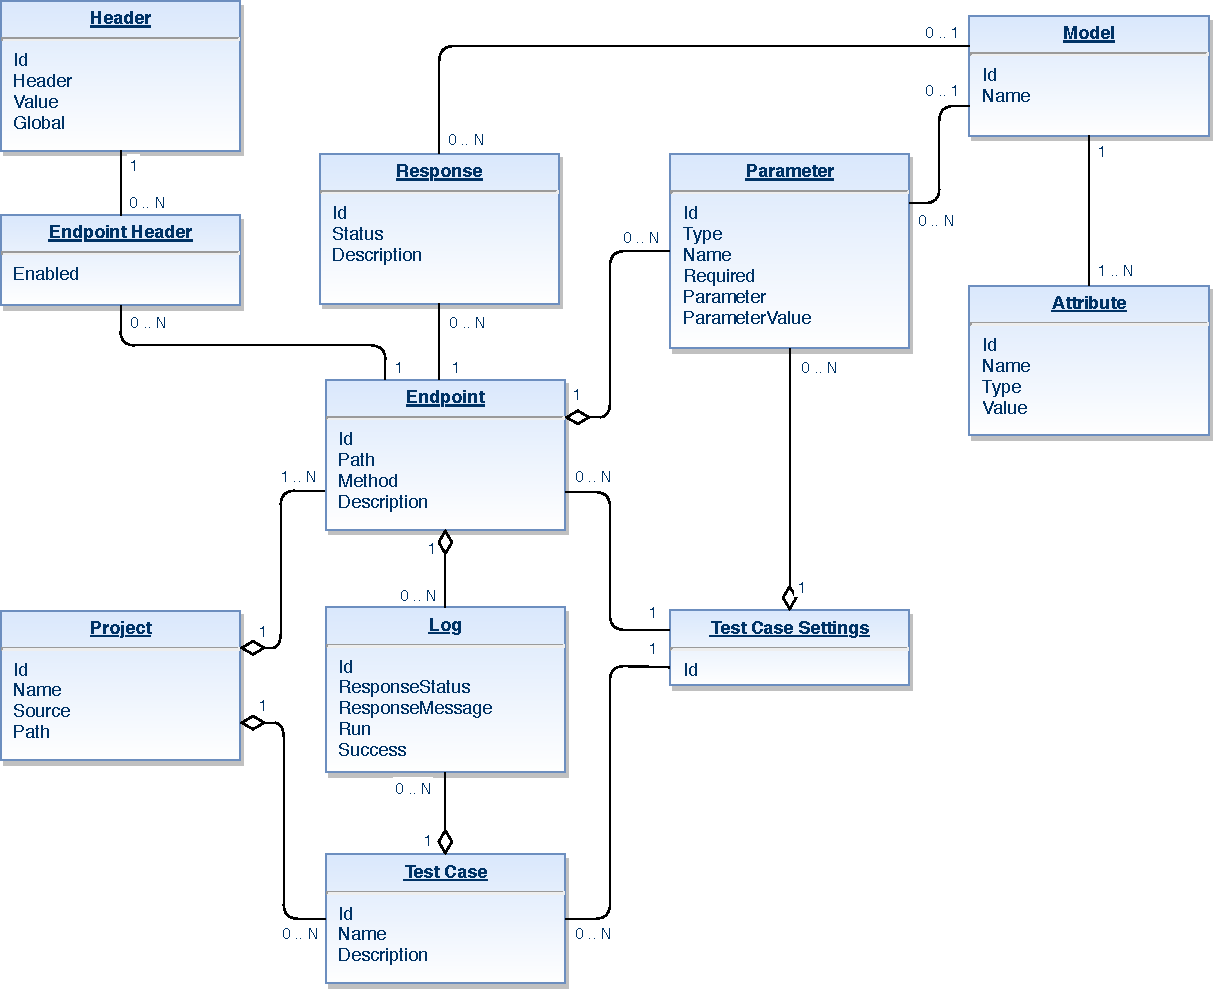
\includegraphics[scale=0.7]{./figures/erd.pdf}
	\caption{The~ER Diagram that describes how the~entities relate to~each other within the~application.}
\end{figure}

In~addition, the~application contains test cases. Test cases consists of~unspecified amount of~endpoints that can have
separate settings -- custom values of~parameters or~models, for~each test case. In~addition, both the~endpoint and~test cases will contain
logs of~previous test runs, to~provide users information about the~tests that were executed in~the~past, and~their results.


\section{Requirements for~the~Restty Application}
As~mentioned earlier, the~aim of~the~thesis is to~create an~application that
allows to~test endpoints of~interfaces of~other applications
as~well~as to~create extensive test cases from~said interfaces. The~interface
that should be tested will be provided via the~Swagger's JSON file which
contains all necessary information about~the~interface. Therefore the~Restty has
to~allow the~users to~choose the~application's interface upon which the~Restty will work.
 If the~interface and~its endpoints is successfully loaded
and~the~data are persisted in~the~database, the~user will be
redirected to~the~dashboard which will display basic statistics about
the~current state of~the~endpoints and~test cases.

From~the~dashboard the~users will be able to~navigate to~the~overview of~all
interface's endpoints, their details, configurations and~past test runs.
In~addition, the~users should be able to~navigate to~the~similar overview
with~test cases, which the~users can create using the~Restty's Test Case
Creator (TCS). The~TCS should allow create test cases that can combine various
endpoints and~other test cases. To~clarify, it should be possible to~test
an~API's endpoint and~use its output as~an~input of~another endpoint.

\section{Design drafts}
As~mentioned earlier, the~design drafts were created to~reveal any clashing visual
elements before writing the~code. However, even though the~thesis presents the~final drafts
of~the~application, it is still possible that parts of~the~design will be changed during
the~development process.

\subsection{Designing the~Project Explorer}
The~entry point of~the~application should be the~Project Explorer. The~Project
Explorer should allow users to~create and~manage the~projects created within
the~Restty. Each project should have a~unique name which distinguishes it
in~the~application. When the~project is created by~the~user, besides its name,
it needs to~have specified a~source of~the~project's endpoints. As~a~source
(in~form of~a~URL) is considered Swagger JSON with~information about
the~project's interface. The~source should be then passed to~the~Restty's
backend that should make an~request for~the~interface, parse the~request's
response and~persist the~information about interface's endpoints and~models
to~the~database. If~the~project information are successfully persisted
in~the~Restty's database, the~user should see the~newly added project and~its
attributes, such as~amount of~endpoints and~test cases, in~the~Project
Explorer's list table.

\begin{figure}[!hbt]
	\centering
	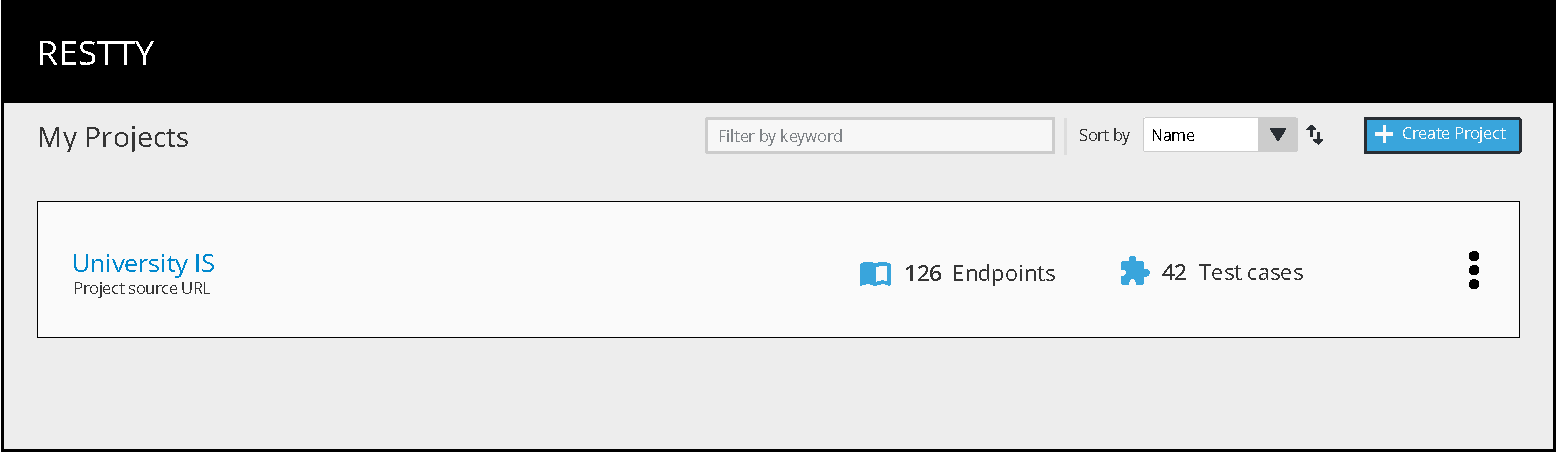
\includegraphics[scale=0.55]{./designs/project-explorer.pdf}
	\caption{The~Project Explorer that contains list of~projects created
	in~the~Restty application.}
\end{figure}

Overall, the~list table should show the~users some basic information about their
projects and~should allow them to~manage them. Finally, by~clicking on~the~list
item the~users should be redirected to~the~specified project's dashboard.


\subsection{The~Project Dashboard}
The~dashboard is the~entry point of~each specific project. It consists
of~a~horizontal and~vertical navigation bars, donut charts and~tables that
contains latest information about the~project. To~keep things simple,
the~horizontal navigation bar should allow users to~swiftly switch between
projects without the~need to~access the~Project Explorer. On~the~other hand
the~vertical navigation bar should allow users to~quickly navigate between
the~project's endpoints, test cases and~settings.

However, the~main aim of~the~Dashboard is to~show the~current state
of~the~project to~the~user. Which is achieved by~showing the~user two donut
charts and~two tables. The~donut charts displays the~state of~the~project's
endpoints and~test cases -- how many of~them were successfully (or~not) tested,
or~if~they were tested at~all. The~tables on~the~other hand shows the~user
the~information about~the~recent API or~test runs. The~Recent table shows
the~user last five runs no matter if they were successful or~not. Whereas
the~Failures table shows the~user unsuccessful runs only, if there are any. From
there on~, using the~navigation bar or~the~quick navigation in~the~tables, user
can start exploring the~endpoints or~the~tests.

\begin{figure}[!hbt]
	\centering
	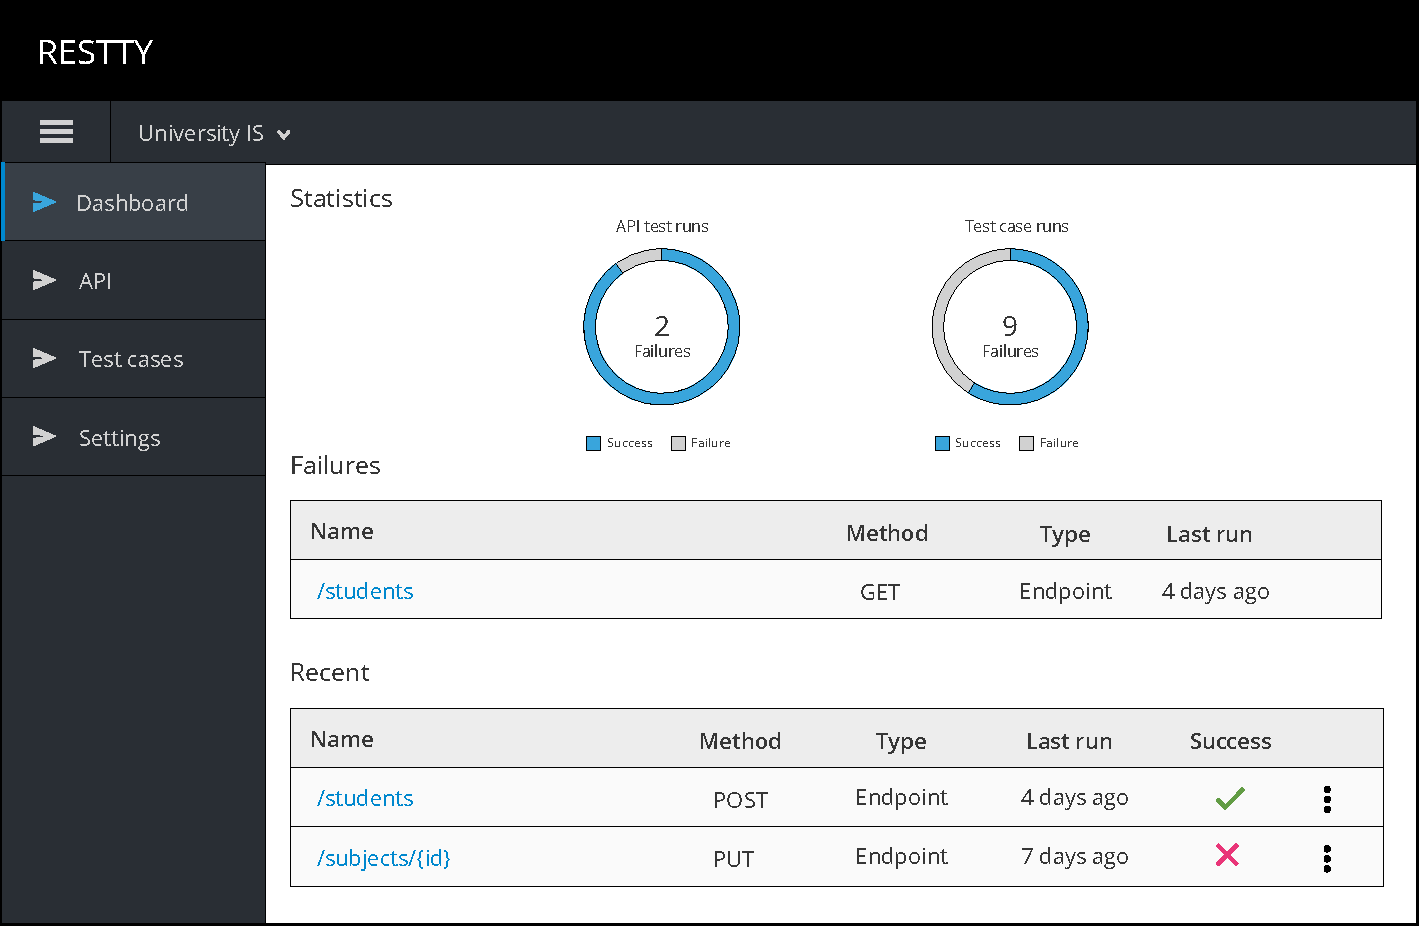
\includegraphics[scale=0.6]{./designs/dashboard.pdf}
	\caption{The~dashboard of~a~project with~lastest information about test runs.}
\end{figure}

\subsection{Exploring the~Endpoints}
Once the~users start working with~the~application, they should be able to~view,
manage and~run the~API endpoints they imported. However, as~explained
in~the~section~\ref{frameworks}, many applications which provide an~overview
of~the~endpoints does not scale well enough if they have to~display a~large
number of~the~endpoints. To~address this issue, the~Restty puts the~endpoints
into filterable list table with~a~simple expansion for~each item. 

Each item contains information about its last test run and~its success.
Moreover, the~item's expansion contains the~details of~the~item's particular
endpoint such as~request headers, path variables, parameters and~responses.

\begin{figure}[!hbt]
	\centering
	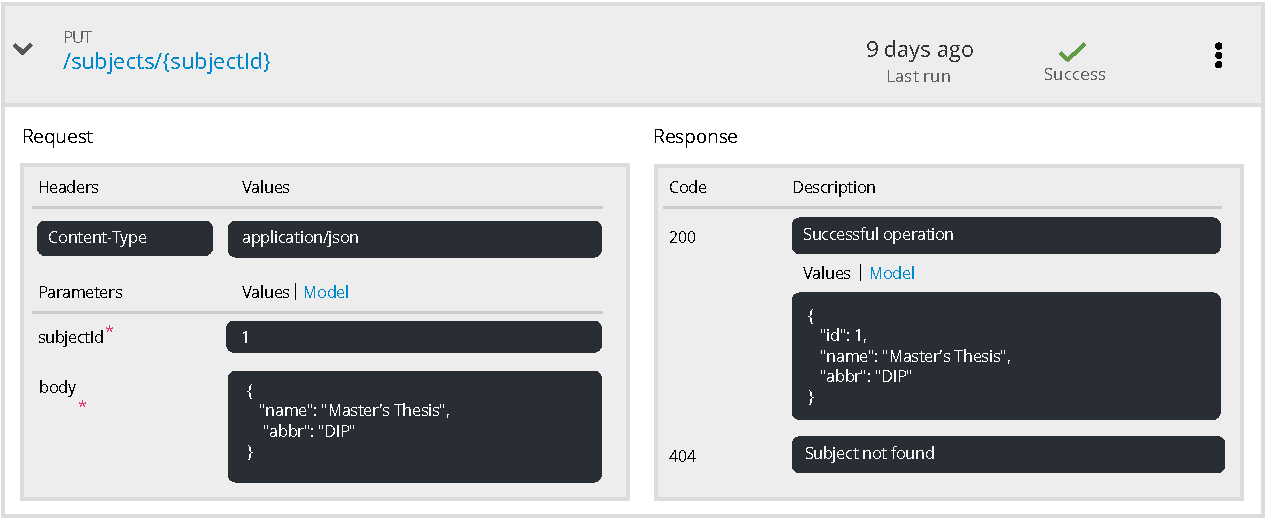
\includegraphics[scale=0.7]{./designs/api-list.pdf}
	\caption{Expanded API endpoint in~the~endpoint's list table.}
\end{figure}

In~addition, when clicking on~the~endpoint's name, its detail is displayed.
The~detail consists of~a~tab view with~three tabs. The~first tab is similar to~the~list item's extension,
showing the~information about request and~responses. The~next one is contains a~configuration that
allows to~make changes to~the~endpoint e.g. changing the~request params, body or~headers. The~last
tab contains records of~previous test runs, so that users know in~which point the~endpoint stopped working
or~when was the~endpoint's code fixed.

\subsection{The Test Cases}
Even though it is important to~enable users to~work with~the~endpoints directly,
the~main focus of~the~Restty is to~test cases. When users view the~test cases page,
they should be able to~manage them. The~management of~the~test cases is outlined using
the~table with~filtering, sorting and~pagination components. Moreover, each item in~the~table
contains basic information about~the~specific test case (e.g. the~date of~last run, its success etc.).

Upon clicking on~the~test case's name, its detail is shown in~a~similar fashion as~the~endpoints detail.
The~view consists of~a~tab view, in~which the~most important tab is the~configuration tab -- containing
the~Test Case Creator (TCC). The~design of~tCC is based on~canvas, which is a~HTML~5 element that allows
for~dynamic, scriptable rendering of~2D shapes and~bitmap images. TCC was designed as~an~dynamic editor that
allows users to~build test cases using various endpoints an~other test cases. The~idea behind it is that the~users
will be able to~construct complex test cases in~the~same way as~they would create a~linked list\footnote{
A~linked list is a~linear collection of~data elements, in~which linear order is not given by~their
physical placement in~memory. Instead, each element points to~the~next. It is a~data structure
consisting of~a~group of~nodes which together represent a~sequence.}.

\begin{figure}[!hbt]
	\centering
	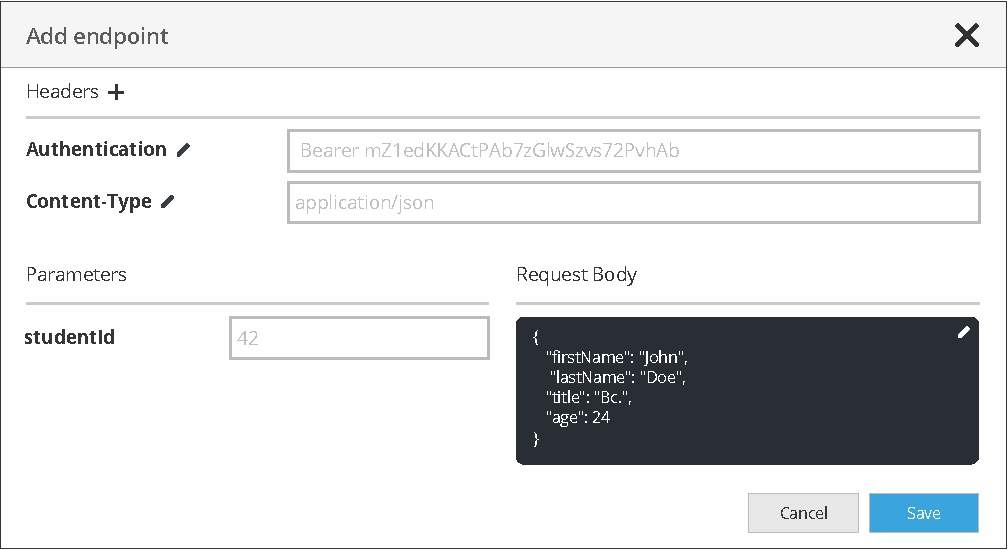
\includegraphics[scale=0.7]{./designs/add-endpoint.pdf}
	\caption{A~modal window that appears when adding first endpoint to~the~canvas.}
	\label{fig-add-endpoint}
\end{figure}

The~TCC consists of~several parts. All of~them together allow users to~model desired
test cases using the~drag and~drop functionality. To~clarify how it works, consider an~example
as~shown in~the~figure~\ref{fig-test-case}. In~the~figure, using the~drag and~drop functionality was
inserted several endpoints from~the~list to~the~canvas. When the~endpoint is dropped, a~modal window
with~the~endpoint's details appears. Note that the~window is prefilled with~the~endpoint's details,
loaded from~its configuration.

However, it is important to~notice that the~behavior specified above is applied only to~first
endpoint that is added to~the~canvas. For~the~following endpoints, the~input data is
automatically derived from~the~previous endpoint output. Once again, consider an~example
from~the~figure~\ref{fig-test-case} that demonstrates how the~data are passed bewteen the~endpoints.
In~the~beginning a~student resource is found or~created and~afterwards immediately deleted, testing 
the~deletion of~the~student resource.

\begin{figure}[!hbt]
	\centering
	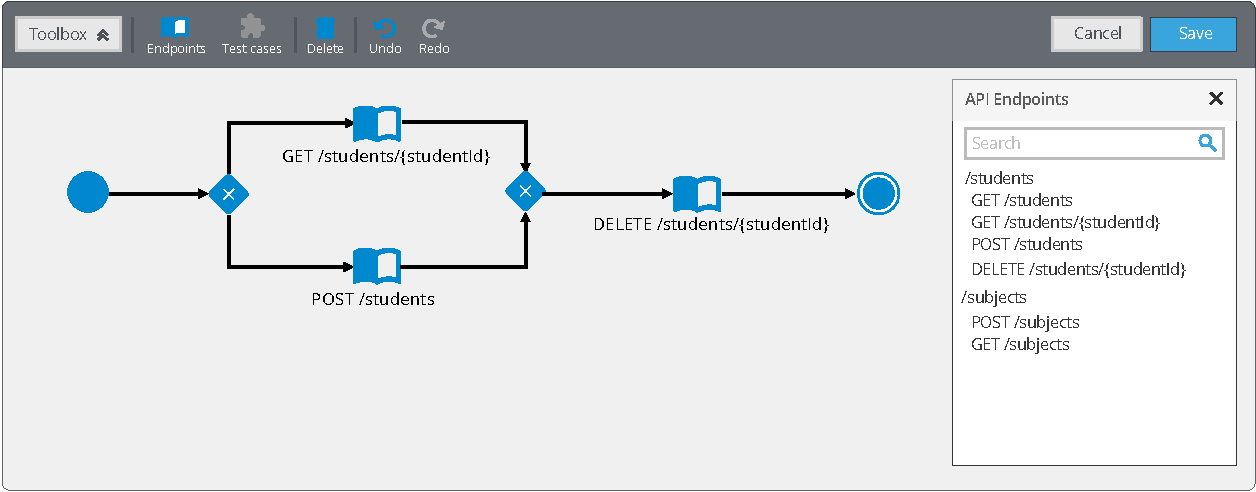
\includegraphics[scale=0.65]{./designs/test-case.pdf}
	\caption{The~TCC with~an~example of~a~test case.}
	\label{fig-test-case}
\end{figure}



% ===============================================================================



\chapter{Implementation and Testing}
The~chapter covers the~implementation of~the~Restty application, based on~the~designs presented
in~the~previous chapter, and~its testing using the~Red Hat JBoss BPM Suite application as~a~source
of~API endpoints to~test. Backend of~the~application is implemented using Java~8, MVC framework
Spring Boot, persistence framework Hibernate 5 and~in~memory database H2. The~frontend is implemented using
Angular~5, TypeScript language and~the~web framework PatternFly.

\section{Separation of Concerns}
Before diving into the~implementation, it is important to~specify the~separation of~concerns between
the~presentation layer (frontend), and~the~data access layer (backend) of~the~application. 
The~frontend is primarily implemented using~Angular while backend is implemented using~Spring Boot. Combining
these frameworks allows to~create a~minimal, but runnable, application with as~little dependencies and~setup as~possible.

Therefore by~following the~separation of~concerns principle, the~application is split into separate Maven modules for~the~frontend
and~backend, where each module has its own POM\footnote{A~Project Object Model (POM) is the~fundamental unit of~work in~Maven.
It is an~XML file that contains information about the~project and~configuration details used by~Maven to~build the~project.} configuration
file linked to~the~parent configuration file. To~build the~Angular application with~Maven, the~frontend's POM file have to~contain 
the~Frontend Maven Plugin dependency, which is needed to~install prerequisities needed by~the~application and~to~keep
the~frontend and~backend builds as~separate as~possible. However, even with~the~Frontend Maven Plugin the~Angular application will not
ended up in~the~final jar. To~ensure that, the~packaged Angular application have to~be added to~backend's resources. This whole approeach
ensures the~separation of~concern principles and~allows the~whole application (frontend and~backend) to~be build using Maven's install command only.



\section{Structure of the Frontend}
When implementing an~the~application, the~most important task is to structure the~application's code
the~right way. Ideally, the~whole application should be a~tree of~components that implement clearly
defined inputs and~outputs, and~minimaze \uv{two-way} databinding. That way, it is easier to~predict
when data changes and~what the~state of~a~component is.

When developing Restty, the~goal was to~create an~application that is scalable and~consists
of~reusable, well encapsulated components that are easy to~maintain and~refactor. To~follow these
rules the~application was divided into~three parts, as~can be seen in~the~figure~\ref{fig-layout}.

\begin{figure}[!hbt]
	\centering
	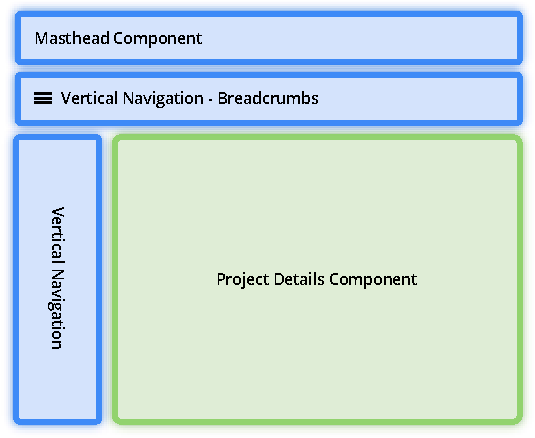
\includegraphics[scale=0.7]{./figures/layout.pdf}
	\caption{The~structure of~a~Restty's main layout components.}
	\label{fig-layout}
\end{figure}

The~only component that is always present is the~Masthead that serves as~an~app's header, containing
the~Restty's name. It is purposely made using the~tall option of~the~PatternFly framework to~accommodate
for~larger app's logo. Following the~design, if the~users open a~project, the~rest of~the~components appears, 
with~one of~them being the~global navigation that is displayed on~the~left. While vertical navigation menus
generally consume more space than their horizontal counterparts, they have become popular as~desktop monitors
move to~\uv{wide-screen} formats. 

Moreover, vertical navigation supports common left to~right flow
and~navigation categories are easily differentiated from~other information that may exist in~the~header area
of~the~application. Which in~Restty's case contains a~hamburger menu and~a~breadcrumbs navigation. 
The~hamburger menu is always visible in~the~top left corner and~allows to~use the~vertical navigation even
on~small devices using \textit{@media} queries and~PatternFly's \textit{navbar-collapse} class.

\vspace{1mm}
\begin{lstlisting}[caption=Media queries on the .navbar-collapse class that enables the~navbar
to~work even on~small devices., style=dp-default]
@media (min-width: 768px) {
	.navbar-collapse.collapse {
		display: block !important;
		height: auto !important;
		padding-bottom: 0;
		overflow: visible !important;
	}
}

.collapse {
	display: none;
}
\end{lstlisting}

Breadcrumbs displays a~users location within an~application hierarchy and~act as~a~resource to~help users navigate more
efficiently and~provide additional context. Note that the~breadcrumbs originally were not part of~the~designs. They
replaced a~context selector that should allow for~quick changing between various projects, but it was decided that
the~breadcrumbs are more useful to~the~user as~the~secondary navigation items like tables are not always exposed.

The~last component in~the~layout is the~\textit{ProjectDetailComponent} that creates a~container for~all subpages,
such as~endpoint and~test cases tables, details etc. The~subpages are displayed using routing which is a~technique
that can interpret a~browser URL as~an~instruction to~navigate to~a~client generated view.

\begin{lstlisting}[caption=Solution of~routing the~subpages in~the~\textit{ProjectDetailComponent}.,
style=dp-default]
// Handles navigation bar clicks
onItemClicked($event: NavigationItemConfig): void {
	this.contentView = $event.title;
	if ($event.title === 'Dashboard') {
		this.contentView = null;
		this.router.navigate(['projects', this.project.id]);
    } else if ($event.title === 'API') {
      this.router.navigate(['projects', this.project.id, 'api']);
    } else if ($event.title === 'Test cases') {
      this.router.navigate(['projects', this.project.id, 'test-cases']);
    } else if ($event.title === 'Settings') {
      this.router.navigate(['projects', this.project.id, 'settings']);
    }
}
\end{lstlisting}

\section{Parsing the Swagger's JSON}
When creating the~project within~the~Restty, the~application consumes Swagger's API file and~parses the~information
about project's interface from~it. As~can be seen in~the~listing~\ref{lst-swagger-json} the~content of~the~file may be extremely
large and~complicated. 

Initially the~source of~the~file is passed to~the~backend when creating the~project, in~which the~\textit{createProject(ProjectDto projectDto)}
method in~the~implementation of~\textit{ProjectService} handles the~project creation. At~first, the~content of~Swagger's file is fetched
using the~Spring's \textit{RestTemplate} class and~then it is parsed to~Data Transfer Objects (DTO) of~which, the~database entities are created.

\vspace{1mm}
\begin{lstlisting}[caption=Parsing the~address of~the~test server from~Swagger's API file,
style=dp-default, language=Java]
ObjectMapper mapper = new ObjectMapper(_;
JsonNode rootNode = mapper.readTree(json);

String scheme = JsonUtils.getScheme(rootNode);
String host = JsonUtils.getPathValue(rootNode, HOST_PROPERTY, false);
String basePath = Objects.toString(JsonUtils.getPathValue(rootNode, "basePath", false), "");
if (StringUtils.isBlank(scheme) || StringUtils.isBlank(host)) {
	this.basePath = source.substring(0, source.lastIndexOf("/") + 1) + basePath;
} else {
	this.basePath = scheme + host + basePath;
}
\end{lstlisting}

The~file contains various information about the~project and~its API, but for~the~Restty's purposes it is important to~parse only~the~information
about~the~test server, endpoints and~the~models. The~information about test server is stored inside the~\textit{host}, \textit{basePath} and~\textit{schemes}
attributes which, once combined, creates a~complete path~that will be used as~default when making API calls. Note that according to~Swagger's specification,
the~\textit{host} and~\textit{scheme} can be omitted for~a~more dynamic association. In~that case, the~host and~scheme used to~serve the~API
documentation will be used for~API calls. 

Once the~information about the~test server are parsed, the~application proceeds to~parsing the~data for~the~entities for~which it needs to~process two
attributes --~\textit{paths} and~\textit{definitions}. The~paths consist of~list of~objects where each object represents particular endpoint. In~addition,
each endpoint contains objects represented by~HTTP methods that are allowed for~the~particular endpoint. Finally, each HTTP~method object contains the~detailed
information about~the~endpoint like its description, parameters or~responses. On~the~other hand, the~definitions consist of~a~list of~objects that represents
entities used~within~the~imported project's API. These definitions are then referenced from~the~endpoints as~parameters or~response bodies.

\vspace{1mm}
\begin{lstlisting}[caption=Parsing the~API's model definitions from~the~Swagger's API file.,
style=dp-default, language=Java]
ObjectNode definitionsNode = JsonUtils.getObjectNode(rootNode, "definitions", false);
	if (definitionsNode != null) {
		definitionsNode.fields().forEachRemaining(definitionNode -> {
			ModelDto model = new ModelDto();
			model.setName(definitionNode.getKey());
                
			ObjectNode propertiesNodes = 
				JsonUtils.getObjectNode(definitionNode.getValue(), "properties", false);
			if (propertiesNodes != null) {
				propertiesNodes.fields().forEachRemaining(propertyNode -> {
					AttributeDto attribute = new AttributeDto();
                    attribute.setName(propertyNode.getKey());

                    String type = 
                    	JsonUtils.getPathValue(propertyNode.getValue(), "type", false);
                    if (StringUtils.isNotBlank(type)) {
                    	attribute.setType(type);
                        model.addAttribute(attribute);
                   	} else {
                    	String modelName = 
                    		JsonUtils.getPathValue(propertyNode.getValue(), "ref", false);
                        if (StringUtils.isNotBlank(modelName)) {
                        	attribute.setType(modelName.substring(modelName.lastIndexOf('/') + 1));
                           	model.addAttribute(attribute);
                        }
                    }
            	});
            }

            models.add(model);
    	});
	}
\end{lstlisting}

\section{Implementation of the API Testing}
This section contains the~details about implementation of~the~cornerstone of~the~whole application 
--~how the~test cases are created and~how they are, along with~endpoints, run. By~default, users can run
the~endpoints straight away but they most likely will not work. That is because the~application does not know
the~parameter values required by~the~endpoints. Therefore users are needed to~specify the~parameters of~endpoints
to~be used in~future endpoints or~test cases runs. 

\vspace{1mm}
\begin{lstlisting}[caption=Frontend's implementation of~setting the~parameter's value in~which\, all logic is handled by~the~matching
TypeScript file., style=dp-html]
<div class="flex-info-left request-params bold">
	<app-edit-param (paramEditEvent)="refreshOnParamEdit($event)" [parameter]="parameter">
	</app-edit-param>
	<div class="edit-parameter inline-block">
		<span class="pf pficon-edit clickable" (click)="createModal('#editParamModal', parameter.id)">
		</span>
	</div>
	<div class="inline-block">
		<span>{{parameter.name}}</span><br>
		<span class="font-size-sm">(query)</span>
	</div>
</div>
\end{lstlisting}

Once all parameters required by~the~endpoint are specified, the~users may run the~test using appropriate button.
The~button is connected to~a~listener, which, on~click, triggers a~REST API call to~the~backend with~the~id of~the~endpoint
that should be tested. On~the~backend, the~request is handled by~the~\textit{EndpointController} that
finds all available information about said endpoint and~passes it~to~the~appropriate service that handles the~test.

\vspace{1mm}
\begin{lstlisting}[caption=The~implementation of~a~test run in~backend's service.,
style=dp-default, language=Java, label=lst-test-run]
RestTemplate restTemplate = new RestTemplate();
HttpHeaders headers = new HttpHeaders();
endpoint.getHeaders().stream().filter(header -> header.getEnabled()).forEach(endpointHeader -> {
	headers.add(endpointHeader.getHeader().getHeader(), endpointHeader.getHeader().getValue());
});

List<Parameter> pathVariables = endpoint.getParameters()
	 .stream()
    .filter(pathVariable -> ParamType.PATH.equals(pathVariable.getType()))
    .collect(Collectors.toList());

String path = endpoint.getProject().getPath() + endpoint.getPath();
String resolvedPath = resolvePathVariables(path, pathVariables);
            
Optional<Parameter> body = endpoint.getParameters()
	.stream()
    .filter(parameter -> ParamType.BODY.equals(parameter.getType()))
    .findFirst();
    
JSONObject jsonBody = new JSONObject();
if (body.isPresent()) {
	body.get().getModel().getAttributes().forEach(attr -> {
		jsonBody.put(attr.getName(), attr.getValue());
	}
            
HttpEntity<String> entity = new HttpEntity<>(jsonBody.toString(), headers);
restTemplate.exchange(resolvedPath, endpoint.getMethod(), entity, String.class);
\end{lstlisting}

The~test is implemented using Spring's \textit{RestTemplate} class which allows calling customizable HTTP requests from~the~backend
services. Furthermore, as~can be seen in~the~listing~\ref{lst-test-run}, when the~test is executed, the~logs are created for~the~endpoint or~test case
that was subject of~the~test, keeping the~information about the~run persisted. Finally, the~testing of~test cases is implemented in~a~similar fashion.
That is because in~fact, a~test case is more or~less a~linked list of~endpoints.

However, there is a~slight difference in~the~test cases implementation. Obviously, the~users might want to~use different parameter values for~the~same
endpoint in~different test cases which is not~possible with~the~current implementation of~the~endpoint's parameters. Therefore the~\textit{TextCaseSettings}
class was created. It~links the~endpoint with~specific test case and~copies the~endpoint's parameters to~its own properties which means that by~default,
if the~endpoint is added to~the~test case, it contains the~parameters that were specified in~the~endpoint's configuration. However, the~parameter values
in~the~\textit{TestCaseSettings} class may be modified without it having an~effect on~the~original endpoint's values. Overall, this approach allows the~users
to~create test cases with~specific conditions which results in~better test coverage of~the~tested project's interface.


\section{Testing with Red Hat JBoss BPM Suite}
\label{Testing}
The~testing of~the~application consistes of~two parts. The~first part consisted of~testing the~Restty's REST API
interface using the~cURL and~Postman applications which validated that the~backend of~the~Restty works as~expected.
The~second, more important part, consisted of~manual testing the~application as~a~whole using the~Red Hat JBoss BPM
Suite application's remote interface.

\subsection{Red Hat JBoss BPM Suite's Basic Concepts}
The~Red Hat JBoss BPM Suite is an~open source business process management suite that combines Business Process Management
and~Businnes Rules Management and~enables business and~IT users to~create, manage, validate, and~deploy Business Processes
and~Rules. To~accomodate Business Rules component, JBoss BPM Suite includes integrated Red Hat JBoss BRMS which is a~comprehensive
bussiness automatiom platform for bussiness rules management, business resource optimization, and~complex event processing.

Red Hat JBoss BRMS and~Red Hat JBoss BPM Suite use a~centralized repository where all resources are stored. This ensures
consistency, transparency, and~the~ability to~audit across the~business. Business users can modify business logic and~business processes
without requiring assistance from~IT personnel.

The~application provides tools for~creating, editing, running, and~runtime management of~BPMN process models. The~models are defined
using the~BPMN2 language, but more importantly, they can be created using the~JBoss BPM Suite API which will be subject of~the~testing.
To~briefly point out options of~what BPM Suite can do, using the~API it is necessary to~provide a~bit of~background on~what rules, events
and~processes are about.

A~business process is a~process that describes the~order in~which a~series of~steps need to~be executed, using a~flow chart. Next, the~events
specify moments in~the~execution process. The~events are fired by~the~BPM's engine during graph execution. An~event is always relative to~an~element
in~the~process definition. Last but not least, a~business rule is a~rule that defines or~contrains some aspect of~process and~always resolves to~either
true or~false. In~other words, rules are linked with~the~process models to~enforce the~correct policies at~each process step.


\subsection{Testing the Restty}
As~mentioned earlier, the~testing was divided into two parts. The~first part was focused on~testing Restty's REST API using
cURL at~first and~Postman later for~more complicated API calls. The~API consists of~several endpoints which are managed
by~appropriate controllers on~the~backend. In~this~section, the~focus will be on~testing the~\textit{ProjectController}
that handles all endpoints, in~which the~path starts with~\textit{/api/projects}.

When starting the~application, the~users will come in~first contact with~projects dashboard e.g. it was needed to~create an~endpoint
that would find all existing projects in~the~Restty application. In~the~listing~\ref{lst-findAll} can be seen the~code used for~testing
the~said endpoint, returning the~list of~all projects within~the~application. 

\vspace{1mm}
\begin{lstlisting}[caption=Testing the~\textit{/api/projects} endpoint using cURL.,
style=dp-default,label=lst-findAll]
curl http://localhost:8081/api/projects
[
	{
		"id": 20,
		"name": "swagger-models",
		"source": "http://petstore.swagger.io/v2/swagger.json",
		"tests": 1,
		"endpoints": 20
	}
]
\end{lstlisting}

As~can be seen~in~the~listing~\ref{lst-findAll}, the~project with~BPM Suite's API is missing, therefore it is needed to~create it using
the~same endpoint as~for~finding the~projects within~the~Restty, but with~the~POST method this time. In~the~listing~\ref{lst-createBPM}
can be seen an~example of~such API call and~its response.

\vspace{1mm}
\begin{lstlisting}[caption=Testing the~creating of~an~project within~the~Restty.,
label=lst-createBPM, style=dp-default, language=XML]
curl --request POST \
  --url http://localhost:8081/api/projects \
  -d '{
  	"name": "bpm-suite", \ 
  	"source": "http://localhost:8080/kie-server/services/rest/server/swagger.json" \
  }'
\end{lstlisting}

Once~the~BPM Suite's project is created, it is possible to~step up in~the~testing process, meaning to~test the~application as~a~whole using
remote interface provided by~the~project. In~particular, for~testing purposes was imported BPM's process server execution module which allows
users to~communicate with~the~process server through REST API. The~first step might be to~test simple GET request, for~instance
the~\textit{/server/containers} which retrieves containers deployed to~the~test server. After the~test is completed, the~user is informed about
its result using a~PatternFly's notification. This process may be repeated multiple times for~multiple endpoints furthermore testing the~application.

However, the~functionality to~test separate API endpoints is provided by~many other applications, as~was stated earlier. Therefore it is necessary 
to~properly test the~functionality of~the~test case. Consider a~following test case -- the~user wants to~test a~deletion of~a~process instance. Normally
he would have to~create the~instance manually, retrieve its id and~then delete it using the~id. However, using Restty this can be automated. User may simple
create a~test case and~to~that test case insert two API requests. The~first request would be the~POST request with~parameters filled 
either from~endpoint's configuration or~by~the~user and~the~following request would be DELETE request that would use the~parameters from~the~previous request.
After running the~test, the~user is again informed about its outcome and~most importantly, he does not have to~modify the~test if~he would want to~run it~again
at~some point in~the~future.

\section{Future extensions}
\label{Improvements}
Even though the~Restty makes testing much easier for~developers, it does not reach its full potential within the~thesis.
The~testing is an~extensive discipline therefore the~application has always room for~improvements. To~make it even more usable 
in~practice, the~following extensions were suggested.

\begin{enumerate}
  \item The~logs that stores the~information about previous test runs could contain more information about the~run besides the~response code and~response message.
  It is possible to~save the~exact format of~the~request, its headers, parameters, etc., and~of~the~response.
  \item The~Project Explorer might offer users to~export existing projects or~to~import projects that were previously created.
  \item The~Restty could offer a~migration to~the~newer version of~the~API, for~instance on~the~backend could be implemented a~cron job that would check if
  the~Swagger's API file was changed and~if it has it could offer an~automatic migration.
  \item Finally, the~Restty could create trivial test cases on~its own -- for~instance, the~tests for~deleting a~resource or~testing the~pagination etc., could
  be done automatically, saving time for~the~developers. 
  \item The~test cases can be extended to~allow users create conditions. For~instance, the~test case could contain a~request that would tried to~find
  a~requested resource. If~the~resource does not exist, it~could be created by~using another appropriate request.
\end{enumerate}

Obviously, the~extensions stated above are not the~only things that can be added to~the~application. It is always possible to~optimize,
the~application itself both in~terms of~performance and~user experience.

\chapter{Conclusion}
The~aim of~the~thesis was to~design and~develop an~application that will allows its users
to~test API endpoints of~other applications and~to~create extensive test cases from~said endpoints.
As~a~part of~working on~the~above goal, I studied the~topics of~Web Services, in~particular the~RESTful
Web Services and~their application programming interfaces. On~top of~that I studied the~technologies needed
for~the~development of~the~application and~conducted a~research on~existing API testing solutions.

In~Chapter~\ref{Design}, I designed a~custom solution of~the~problem using~the~design integrity of~the~PatternFly
framework. The~designs, that were several times consulted in~Red Hat, were used to~reveal any clashing visual elements
or~design flaws before writing the~code. After several reworks and~improvements they wre used as~a~basis
for~the~development of~the~application.

The~development consisted of~two parts -- building the~frontend and~a~backend as~separate sections, following the~Separation
of~Concerns principles. The~achievement is that the~backend of~the~application is fully capable of~parsing the~Swagger's API 
file, running and~managing its endpoints, and~allowing to~create extensive test cases from~said endpoints. In~addition,
the~frontend of~the~application provides clear and~easy to~use interface, even in~case of~large remote interfaces.

Finally, as~stated~in~the~section~\ref{Testing}, Restty was tested on~Red Hat JBoss BPM Suite application, which provided
a~large remote interfaces consisting of~various different endpoints that were used to~reveal any~errors or~bugs in~the~application
and~to~learn more about the~Restty's future improvements, such~as~automatic test case creation or~automatic migrations to~the~newer
versions of~the~remote interfaces. Overall, the~application serves its purpose and~has a~potential to~become the~leading application
for~the~API testing processes and~test automation.



%================================================================================
